\documentclass[UTF8]{ctexart}

\title{From Word Embeddings to Item Recommendation}


\usepackage[super,square,compress]{natbib}%参考文献样式

%调整段间距,在原有基础上增大0.4em
\addtolength{\parskip}{.4em}
%生成书签。同时不是使用方框标识,colorlinks使用颜色标识。如果不想使用颜色,可以改为black.
%书签可有可无。不想用直接删除即可
%colorlinks默认为false, 即使用方框区别链接。为true时使用颜色进行区别。
\usepackage[colorlinks=true,
linkcolor=red,
anchorcolor=blue,
citecolor=green
]{hyperref}

%%%%[dvips]有时候加入这个选项反而会使图片出现空白
\usepackage{graphicx}%图片包
\DeclareGraphicsExtensions{.eps,.ps,.png,.jpg}%对于同名图片的优先顺序调用
\graphicspath{{graphics/}}%设置图片路径为当前路径下的graphics文件夹

\begin{document}
	\maketitle
	\begin{abstract}
		社交网络平台可以对他们的用户群产生的数据进行存档然后在重新使用这些数据为用户提供更好的服务。在这些平台中所提供的服务中其中之一就有推荐服务。推荐系统能够使用各种不同的技术来预测用户未来的偏好。推荐中一个非常流行的技术便是矩阵分解,这是对输入数据采用低秩矩阵的一种近似。与此相似,在自然语言处理中使用的词嵌入方法也是学习输入元素在低维向量空间的表达。注意到词嵌入与矩阵分解的相似之处,同时联系已有的一些将文本处理的技术应用到推荐上的工作, 将Word2Vec's skip-gram技术应用到推荐中。不像以前的一些利用Word2Vec做推荐的工作,使用非文本的特征。本篇工作的目的在于推荐下一个check-in地点,并使用了Foursquare的check-in数据集。结果表明通过使用skip-gram技术对于物品在向量空间进行建模对于做出推荐很有前景。
	\end{abstract}
	
	\begin{center}
		关键词:推荐系统;基于地点的社交网络;词嵌入;Word2Vec; Skip-gram技术
	\end{center}
	
	\section{Introduction}
	社交网络平台(比如,Twitter,Facebook,Foursquare)拥有很多的活跃用户,这些用户通过与平台上的其他用户或平台上的产品或服务进行交互而产生大量的信息。比如,截止2015年12月,在Twitter上每个月有3.2亿的的活跃用户,超过5千5百万的用户使用Foursquare,Facebook有超过10亿的日活跃用户。这些平台能够存档并使用这些产生的信息来更好的服务用户。在社交网络平台提供的最多的其中一个服务便是推荐服务。
	
	推荐系统基于用户以前的一些对于物品的交互对它们未来的偏好进行预测。比如,用户在Foursquare以前的一些check-in信息能够被用在对于用户未来的check-in地点推荐中。正如已经所提及的,拥有用户大量的用户偏好的历史信息。在已有的文献中,这些信息被以几种不同的方式用来做出推荐,比如,通过基于近邻,基于机器学习和基于矩阵分解的方式。近来,由于基于矩阵分解的方法能够很有效地利用对于输入数据的低秩近似来应对大规模的数据集\cite{ma2011recommender},矩阵分解在研究者中获得更多的关注。
	
	与矩阵分解方法相似,词嵌入方法学习输入元素在低维向量空间的表达。它们被用来从大规模的文本数据集学习语言规则和语义信息,并且正在自然语言处理和文本挖掘领域获得更多的关注\cite{musto1441word}。在本篇的工作中,我通过使用Word2Vec\cite{mikolov2013distributed}中的skip-gram word embedding技术来推荐下一个check-in地点。
	
	在推荐系统中使用文本处理技术的效率问题已经在之前的一些工作\cite{gao2012exploring,shin2014recommending,musto1441word}中被举例。\cite{gao2012exploring} 是在Location Based Social Networks(LBSNs)的地点推荐中一个非常先进的方法,它使用基于语言模型的方法。\cite{shin2014recommending}旨在为用户推荐哪一个博客去关注。它使用了Word2Vec对基于单词的特征进行建模,也就是说,标签。\cite{musto1441word}利用了三种不同的词嵌入技术,其中一种便是Word2Vec,来对MovieLens与DBook数据集做出推荐。它利用了从维基百科收集的关于物品的文本数据。
	
	在本篇工作中,我利用了Word2Vec's skip-gram 技术对LBSNs进行推荐。与之前一些利用Word2Vec进行推荐不同\cite{shin2014recommending,musto1441word},我使用了非文本的特征,叫做用户的历史check-in. 在评价环节我使用了在之前的一些工作\cite{ozsoy2014multi,gao2012exploring}所使用过的数据集,Foursquare check-in数据集。
	
	本文一下内容结构如下:1,介绍了相关工作;2,解释了Word2Vec与我们所提出的方法;3,给出了实验结果;4,本文总结。
	
	
	\section{Related Work}
	推荐系统通过估计偏好做出对物品的推荐\cite{massa2007trust,tavakolifard2012social}。大致有3类基本的推荐方法:基于内容,协同过滤与混合方法。基于内容的方法利用物品特征和它们的相似度做出推荐。协同过滤方法利用用户过去的偏好决定为用户推荐哪一个物品。混合方法则将这些推荐方法进行混合做出最终的推荐。
	
	除了上面所提及的方法,基于矩阵分解的方法也在推荐系统研究者中获得关注。这些方法使用对于输入数据的低秩近似从而能够处理大规模的数据\cite{ma2011recommender}。在\cite{koren2009matrix}中阐明了矩阵分解能够将物品与用户表示为向量,而这些向量对于推荐则有着很高的相关性。此外,在同样的工作还阐明了这些方法拥有很好的扩展性,很高的准确度与灵活性。已有一些示例工作\cite{ma2008sorec,zheng2010collaborative,liu2013soco,cheng2013you,lian2014geomf}中使用矩阵分解来推荐。在这些工作中,\cite{zheng2010collaborative}与\cite{cheng2013you}有着与我们的方法相同的目标,他们为目标用户推荐地点或是活动,不过在他们的方法并没有使用Word2Vec。
	
	与矩阵分解方法相似,在自然语言处理领域的词嵌入方法学习输入元素在低维向量空间的表达。词嵌入从输入的文本数据集中学习语言规则与语义信息,然后通过一个向量表示词语的意义\cite{musto1441word,arora2015random}. 在\cite{arora2015random}中词嵌入可以通过隐语义分析(Latent Semantic Analysis),主题模型与矩阵分解技术来进行学习。在Word2Vec\cite{mikolov2013distributed}所定义的技术叫做skip-gram和continuous bag of words(CBOW),它们常常在文献中被用来表示词向量(word vectors).
	
	一些推荐方法\cite{shin2014recommending,musto1441word}使用Word2Vec技术来表示基于文本的特征。\cite{shin2014recommending}旨在为用户推荐关注哪一个Tumblr博客。在这个工作中的推荐方法中使用了inductive matrix completion(IMC)。这个方法同时使用了侧面特征(喜欢,转载和标签)与用户过往的偏好。它并不直接使用自然语言处理技术,而是利用Word2Vec计算标签的向量表示,而它们是基于词语的特征。\cite{musto1441word}从经验上评估了三种词嵌入技术并用来推荐,分别叫做Latent Semantic Indexing, Random Indexing 和Word2Vec, 并在MovieLens与DBbook数据集上测试了他们所提出的方法。他们利用维基百科将数据集中的物品映射为文本内容,然后利用文本内容来进行推荐。另一个利用自然语言处理技术的推荐方法是在\cite{gao2012exploring}中提出的Socio-Historical方法。这是在LBSNs的地点推荐中一个很先进的方法。考虑到文本挖掘与社交网络数据集的相似之处,它利用了自然语言处理中的语言模型来进行地点推荐。它可以用或分离或组合的方式对历史偏好与社交网络间的相互联系进行建模。
	
	Word2Vec的技术通常被认为是deep learning技术。比如\cite{salakhutdinov2007restricted,georgiev2013non,wang2015collaborative}几乎没有其他深度学习的方法能够被用来推荐系统中.在\cite{salakhutdinov2007restricted}使用 Restricted Boltzmann Machines(RBM's)来推荐电影。它对物品评分间的相互关系进行建模。\cite{georgiev2013non}通过对用户与用户之间和物品与物品之间的相互关系进行建模扩展了\cite{salakhutdinov2007restricted}。\cite{wang2015collaborative}提出了hierarchical Bayesian模型,该模型通过物品的内容信息与用户过去的偏好信息来进行学习。
	
	在本篇工作中,我利用了Word2Vec的skip-gram技术来为目标用户推荐check-in地点。与之前的一些在推荐中利用Word2Vec\cite{shin2014recommending,musto1441word}不同, 我利用了非文本的特征叫做用户的过往check-ins。
	\begin{figure}
		\begin{center}
			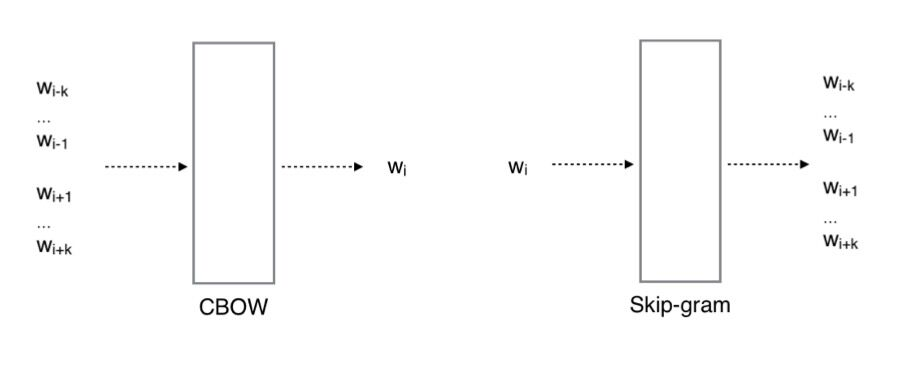
\includegraphics[width=4in]{1}
		\end{center}
		\caption{Word2Vec techniques}
	\end{figure}
	
	
	\section{Recommendation using multiple data sources}
	我们的目标是为目标用户列出将会在未来访问的top-k check-in地点。为此我使用了叫做的skip-gram的Word2Vec技术。在本节中,我将会简短介绍Word2Vec技术并解释了在check-in推荐中如何利用了skip-gram技术。
	
	Word2Vec是Mikolov\cite{mikolov2013distributed,mikolov2013efficient}引进的一组模型。它包含了两类不同的技术,分别叫做skip-grams和(continuous bag od words)CBOW,而它们将生成词嵌入,也就是说,分散的词表示(distributed word representation).词嵌入在一个低维的连续空间中表示词语并且携带了词语的语义与语法信息\cite{li2015word}。而CBOW技术使用当前词附近的一些词来对当前词进行预测,skip-gram技术也是如此。在这这种技术中,都使用了bag-of-words表示,也就是说输入的词语顺序并不会影响结果。
	
	\cite{levy2015improving}阐述了CBOW对来自语境窗口中的词语进行组合的做法,这种做法并不能被简单地表述为分解。但是,\cite{levy2014neural}含蓄地表明skip-gram的矩阵分解做法。分解的word-context矩阵是一个co-occurence矩阵,在文献中常表示pointwise mutual information(PMI).注意到矩阵分解与Word2Vec技术都是对输入数据构建了低秩的一个近似,我打算将Word2Vec的skip-gram技术应用到推荐推荐下一个check-in地点。
	
	我们所提出的方法由以下步骤构成:首先使用skip-gram技术对输入数据进行建模,然后这个模型用到推荐的执行过程中。
	
	\subsection{使用skip-gram技术对输入数据进行建模}
	skip-gram是用来推荐的一种很好的技术:首先,在推荐中使用文本处理技术已经在文献中被例证;其次,skip-gram技术隐式地将输入矩阵进行分解,而矩阵分解技术已经在推荐系统中被发现是很有效的一种方式。最后,skip-gram技术是比CBOW更好的技术,因为它表现的比CBOW技术要好,或是不相上下\cite{mikolov2013distributed,levy2014neural}.
	
	我使用了在gensim工具包实现的skip-gram技术。该实现接受一串句子作为输入,同时这些句子本身也是有一串词语组成。这些词语被用来创建内置的词典,该词典包括了词语和它们的词频。在通过输入数据和词典训练好模型后,输出的是词向量, 这些词向量可以在不同应用中视作为特征[25]。在训练过程中可以就时间与质量的考量对不同的参数进行调整。在评测环节我详细阐述了参数是如何调整以及不同值的效果。
	
	我注意到在skip-gram与推荐过程的几个相似点:第一,在skip-gram技术中的输入数据与推荐过程中所使用的实际上是很相似的。在推荐过程我使用了用户在过去所喜欢或是评分过的物品列表,然后将这些列表分割为单独的一些物品。换句话说,在skip-gram中使用的句子能够被映射为在推荐过程的用户过去的偏好,同时将skip-gram的词语映射为推荐过程的个体物品。第二,skip-gram技术与推荐技术的目的是相似的。skip-gram旨在基于当前单词预测语境词(context word),而推荐系统是基于已经有过偏好的物品行为预测物品。
	
	在传统的推荐过程中,输入数据由三种基本的元素构成:用户,物品与评分。在大部分的算法中,这些元素由用户与物品矩阵所表示,其中的矩阵条目表示评分。在我们的check-in推荐问题中,评分数据被认为是二元数据,比如用户是否check in过一个地点。然后,每个目标用户的过去偏好能够被表示为一个列表的物品(check-in地点)。
	
	受到[8]的启发,我共同使用了用户与物品列表,也就是说,不仅是物品还有所有的用户与这个用户有过交互行为的物品,然后将这些作为skip-gram技术。通过使用skip-gram技术将能够分别获得用户与物品的向量表示。这些向量表示能够被用来决定哪一个物品比其他物品更相似或用户在语境上更接近于哪一个物品。这些向量与相似度可以被用在我们下一步的推荐方法中。
	
	\subsection{使用向量表示进行推荐}
	skip-gram模型提供了词向量,这些词向量的单词在意义上越相似在向量空间中距离越近。在推荐情况下,就不是单词而是物品与用户。skip-gram的输出提供了物品与用户在向量空间的向量表示,且越相似的向量距离越接近。在这个报告中提出了三种不同的使用物品与用户的向量表示的推荐技术:
	
	\textbf{通过k-nearest items进行推荐:}在我们使用k-nearest items(KNI)的推荐方法中,使用了物品与用户向量之间的相似度。在这个方法中,直接找到了目标用户最相似的k个物品。为此使用了向量间的cosine相似度,然后收集到的top-k个物品推荐给目标用户。
	
	\textbf{通过N-nearest users进行推荐:}在使用N-nearest users(NN)的推荐方法中,传统的基于用户的协同过滤被应用到向量表示中。在基于用户的协同过滤中,首先选出与目标用户最相思的一些近邻用户,然后将近邻用户所喜欢过的一些物品推荐给目标用户。与传统方法类似,在NN方法中,首先通过用户的向量间的相似度决定出top-N个近邻,然后选择出这top-N个用户以前所喜欢过的物品。将近邻用户的投票累加起来,就选出了用来为目标用户推荐的top-k个物品。
	
	\textbf{通过N-nearest users 和k-nearest items进行推荐:}这种方法是对之前两种方法的组合。在这个方法中,首先通过用户的向量表示找到top-N个近邻。然后通过在第一步中计算得到的向量表示找到top-k个物品,而这些物品是与目标用户及其近邻间最相似的物品。最后将这top-k个物品推荐给目标用户。
	
	
	\section{Evaluation}
	我们的目标是基于每个用户过去的check-ins然后给用户推荐k个check-in地点。为此我们使用了在\cite{gao2012exploring,ozsoy2014multi}中使用过的Checkin2011数据集。原始数据集是从2011年1月至2011年12月在Foursquare网站收集所得,它包含了11326个用户,187218个地点,1385223个check-ins和47164个朋友链接。不过,在\cite{ozsoy2014multi}中研究人员使用了这个数据集的一个子集,也就是一月份的check-ins作为训练集,并称之为CheckinsJan. CheckinsJan数据集包含了8308个用户,49521个地点和86375个check-ins。在测试环节使用了二月份的check-ins作为测试集,并且目标用户被限制为在一月份与二月份都有过check in行为的用户。目标用户集合包含了7187个用户。在本篇文章所提出的方法也与\cite{gao2012exploring,ozsoy2014multi}进行了比较。
	
	我们通过Precision@k,Ndcg,Hitrate和Coverage metrices对性能进行评测。当给出评估结果时,首先单独计算每个用户的性能评估值然后在计算其平均性能。
	
	Precision@k衡量了输出列表中物品的相关性。公式1表明如何计算Precision。在公式中,$k$表示推荐列表的大小,$tp$表示实际推荐并被使用的物品,$fp$表示实际推荐但并未被使用的物品。
	
	Ndcg(Normalized discounted cumulative gain)就排序角度衡量了推荐列表中物品的相关性。公式2和3分别表明了如何计算Ndcg(Normalized discounted cumulative gain)与Dcg(Discounted cumulative gain)。Idcg值指根据相关性对推荐列表进行排序的最好情况。在公式中,$k$为输出列表的大小,$j$为输出列表中物品所在的位置,$rel_j$表示在位置$j$的物品是否是相关的(true recommendation)。当处于位置$j$的物品是相关的则$rel_j$为$1.0$,否则为$0.0$.
	
	Hitrate衡量了用在在所推荐中至少命中一个的比率。在公式4中,$m$表示其中一个用户,$M$表示所有用户的集合,$|M|$表示用户数。$HitRate_m$表明对于目标用户$m$是否会有一个命中。如果对于一个用户至少有一个true recommendation则$HitRate_m$为$1.0$否则为$0.0$.
	
	收敛性衡量了为用户提供的任何推荐的比率,而其与是否相关无关。在推荐系统中,一些方法可能会为了提高准确度而失去收敛性\cite{bellogin2013empirical,herlocker2004evaluating},这表明收敛性与准确度应该被同时分析。
	
	在本篇报告所提出的方法使用了两个参数:近邻数$N$与推荐列表的大小$k$。\cite{ozsoy2014multi}认为对于CheckinsJan数据集最佳表现值为$N=30$和$k=10$,这些值都在实验中被使用。同时\cite{ozsoy2014multi}也阐明了在所给参数的方法上的上界:对于Precision考量的上界被发现为$0.489$而余下的考量为$1.0$。
	\begin{figure}
		\begin{center}
			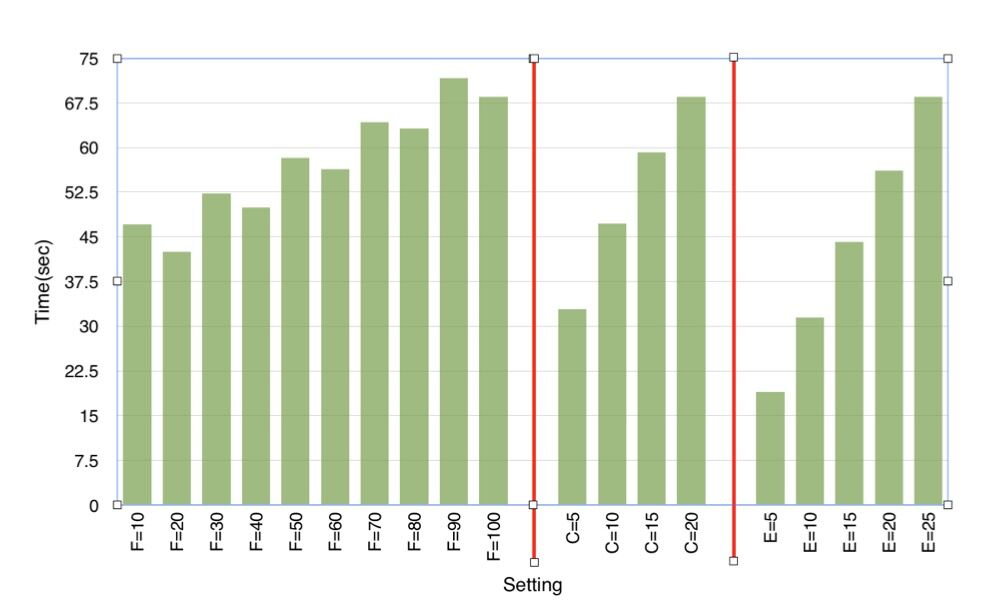
\includegraphics[width=4in]{2}
		\end{center}
		\caption{The time needed to model the input data with skip-gram technique}
	\end{figure}
	
	当输入数据通过skip-gram技术进行建模后在评测几组不同的设定值。在训练中使用的参数在时间与质量上影响着推荐表现[26]。这些参数都是基于gensim toolbox的实现。参数设置的细节及调整方式如下:
	\begin{itemize}
		\item $min\_ word \_count:$ 这个技术忽略词频比该参数还要小的物品。默认值为5.在自然语言处理中,那些仅仅出现几次的物品(词语)被认为是无用的,但是在推荐系统中由于数据很稀疏并且物品仅被观测到几次的情况时极其常见的。为了不漏掉任何一个使用并不平凡的物品,我将参数$min\_word\_count$设置为1.
		\item $size:$参数size表示特征向量的维度,并且它的默认值为100.在[26]中,认为$size$越大则模型越准确,但是需要更多的数据。对于$size$的建议值为几十到几百之间。在我们的实验中这个参数被表示为$feature\_count\left(F\right)$, 并且以10为一个梯度设置为范围为$[10,100]$间的不同值。
		\item $window:$参数window指定了在当前词语与预测词语之间的最大距离,默认值为5.[26]认为它应该足够大以便能够捕捉到词语间的语义联系。在我们的实验中这个参数被表示为$context\_count\left(C\right)$,并且以5为一个梯度范围在$\left[5,20\right]$间的不同值。
		\item $iter:$参数iter表示对于输入数据的迭代次数,默认值为1.在我们的实验中被表示为$epoch\_count\left(E\right)$,并且以5位一个梯度范围在$\left[5,25\right]$的不同值。
	\end{itemize}
	
	对于CheckinsJan数据集的模型训练时间如图2所示。根据图表,当特征数增加时,训练时间大概增加40s至70s。类似地,参数$context\_count$与$epoch\_count$增加时训练时间也会随之增加。总体的结果表明CheckinsJan数据集的模型训练时间少于75s。
	\begin{figure}
		\begin{center}
			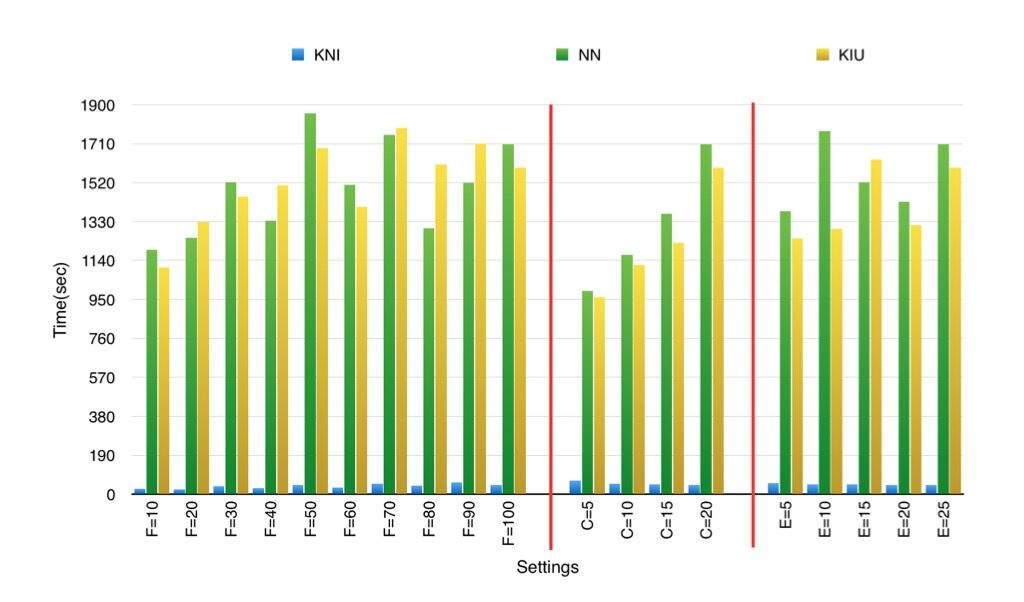
\includegraphics[width=4in]{3}
		\end{center}
		\caption{The time needed to make recommendation using the model created by skip-gram}
	\end{figure}
	
	本文提出的共有3种不同的推荐技术使用了skip-gram训练的模型。这些技术为‘recommendation by k-nearest items(KNI)’,'recommendation by N-nearest items(NN)','recommendation by N-nearest users and k-nearest item(KIU)'. 为所有目标用户做出推荐所花费的时间如表3所示。 图表显示KNI相比其他方法花费更少的时间,因为它直接使用了模型的输出而没有进一步的计算,比如寻找近邻。即便是花费最多时间的方法与参数设置其对CheckinsJan数据集的所有目标不超过1900s。而整个数据集有7187个用户,也就是说在推荐过程中每个目标用户花费的时间不到0.26s。
	
	在表格4-6中展示了所提出方法的推荐表现。对于所有的方法增大$feature\_count$,即向量表示的大小,都能够提高表现。不过当这个参数值超过50时,即使再继续增长提升的效果将变得越不明显。当$context\_count\left(C\right)=5$时该模型将不能够捕捉到物品与用户间的语义相似性。在设置该参数值$C=10$设置更高时,越高则表现越好。对于$context\_count$与$epoch\_count$,参数值的增加仅会对推荐表现产成微弱影响。
	
	根据图表4-6中推荐技术的表现比较,最好的方法是KNI,其次为KIU.这些方法都利用了目标用户对物品的向量表示及其相似度。虽然KNI与KIU都利用了物品向量间的相似度,不过KIU更是额外地利用了目标用户的近邻用户,而这些近邻用户则是由用户向量间的相似度所决定。与KNI相比,在KIU中对于近邻的利用并没有获得很好的推荐表现。这可能表明在CheckinsJan数据集上使用用户向量相似度本身就是没有什么效果。这可能也是在向量空间中用户无法被区分的根源所在,尽管数据集中的用户数并不是很高,仅有8307个用户。
	\begin{figure}
		\begin{center}
			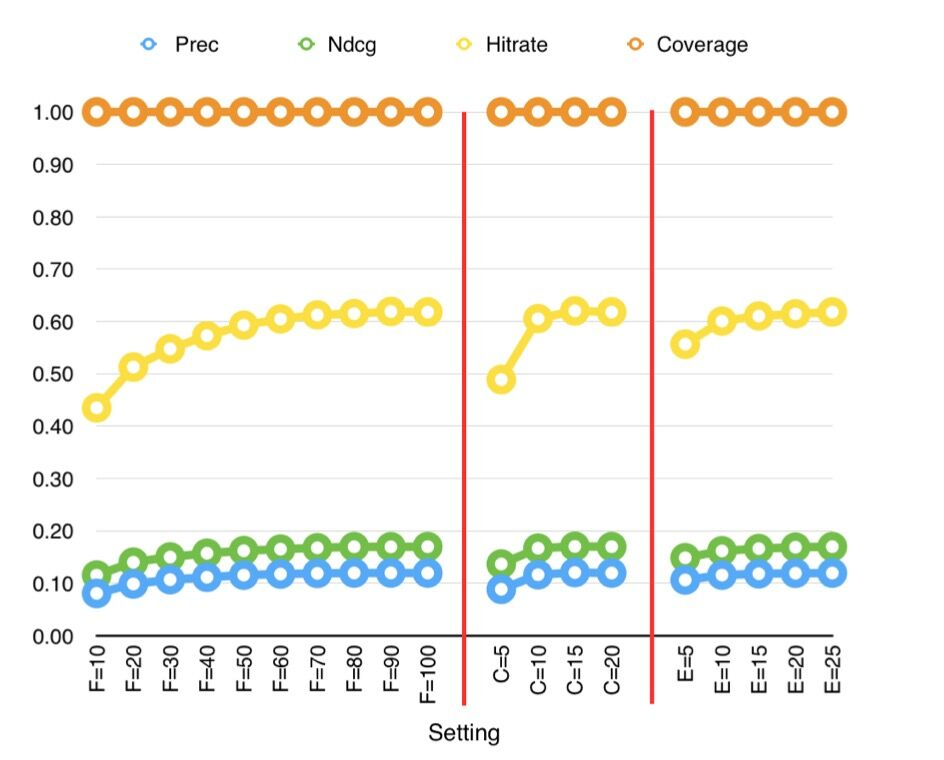
\includegraphics[width=4in]{4}
		\end{center}
		\caption{Performance results of KNI}
	\end{figure}
	
	\begin{figure}
		\begin{center}
			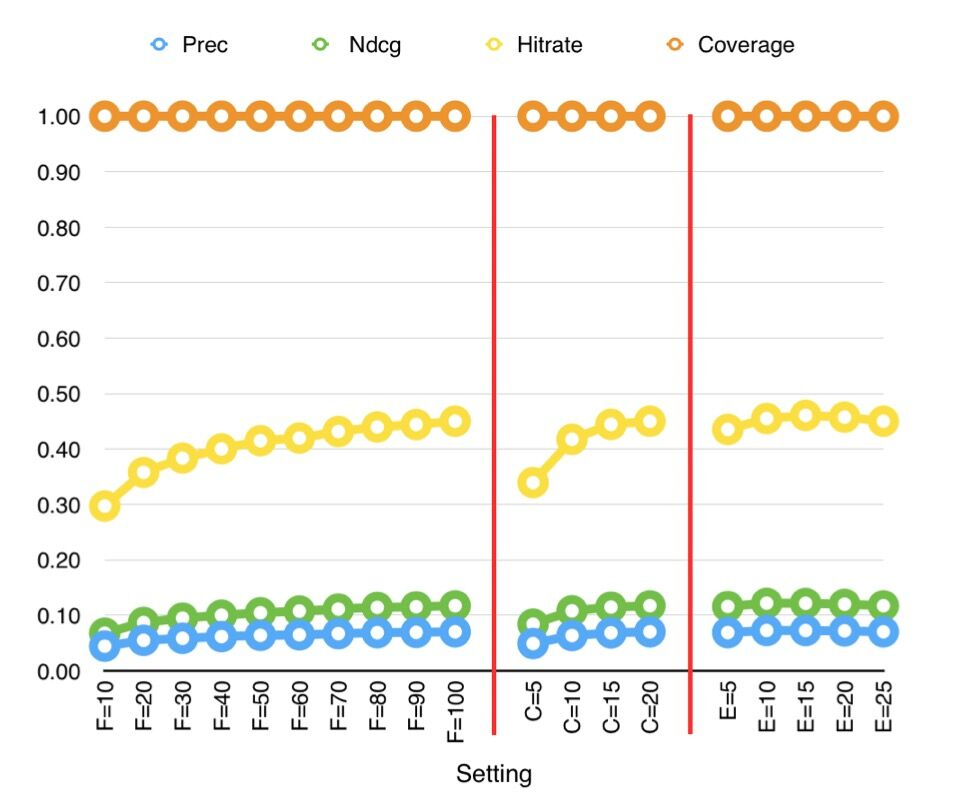
\includegraphics[width=4in]{5}
		\end{center}
		\caption{Performance results of NN}
	\end{figure}
	
	\begin{figure}
		\begin{center}
			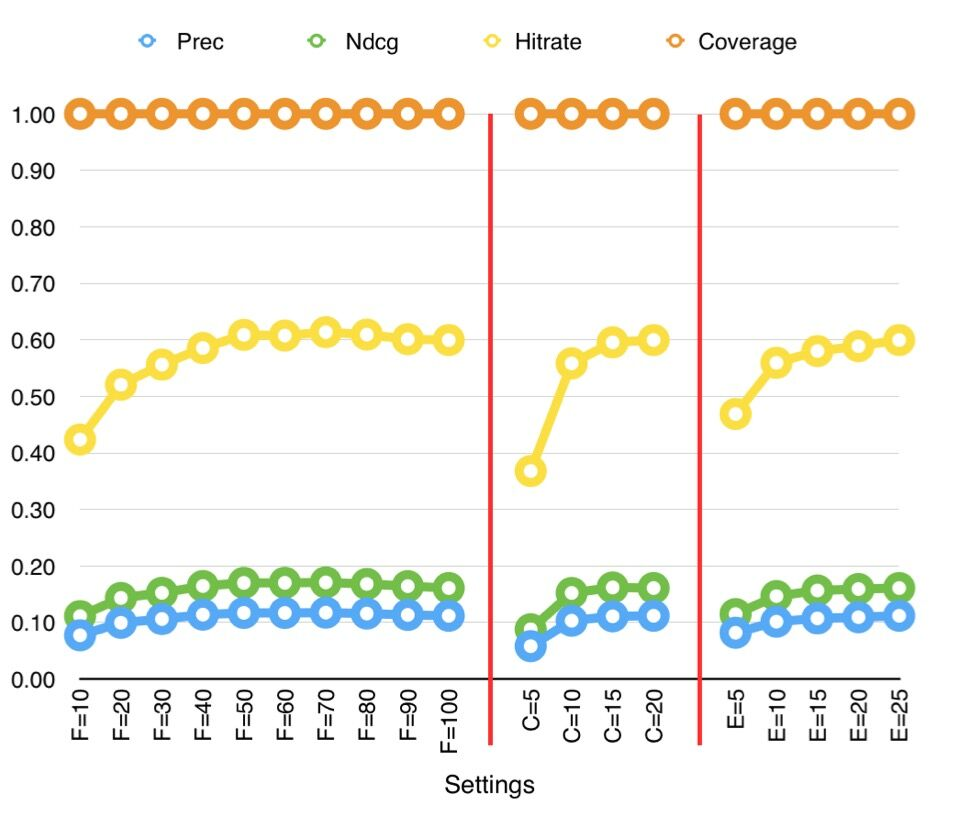
\includegraphics[width=4in]{6}
		\end{center}
		\caption{Performance results of KIU}
	\end{figure}
	
	在表格1中,我将在本篇报告中所提出的方法,即KNI,NN和KIU与已有的一些推荐方法进行了比较。第一个方法便是传统的协同过滤方法,它使用了用户过去的偏好和其相似度。接下来的两种方法来自\cite{ozsoy2014multi},它们基于多重目标的优化技术并将用户过去的偏好与其他一些特征进行了组合,比如用户的家乡,朋友及其相互关系。使用了过去的check-ins和用户的故乡的方法简称为MO-CH,而使用了上面所有提到的特征的方法简称为MO-CFIH。最后的两种方法来自\cite{gao2012exploring},它们使用了来自自然语言处理的一个语言模型进行推荐。这个方法能够对过去的偏好与用户的社会关系进行组合。我使用了两个版本的该方法,其中一个仅使用了用户过去的偏好(Gao-H),另一个使用了过去的偏好与社会关系进行组合(Gao-SH).
	
	
	根据表格\ref{tab:1},在本篇报告所提出的方法,KNI,NN和KIU能够对任何用户进行推荐,也就是说$Coverage=1.0$.表现最好的方法是Gao-H和Gao-SH,这也表明在自然语言处理中的一些方法对于推荐的确有效。就Precision与Hitrate而言,除了\cite{gao2012exploring}的方法,KNI比其他方法的表现都要好。就Ndcg而言,通常一个利用了多种特征的方法会比单一特征的方法要更好。
	\begin{figure}
		\begin{center}
			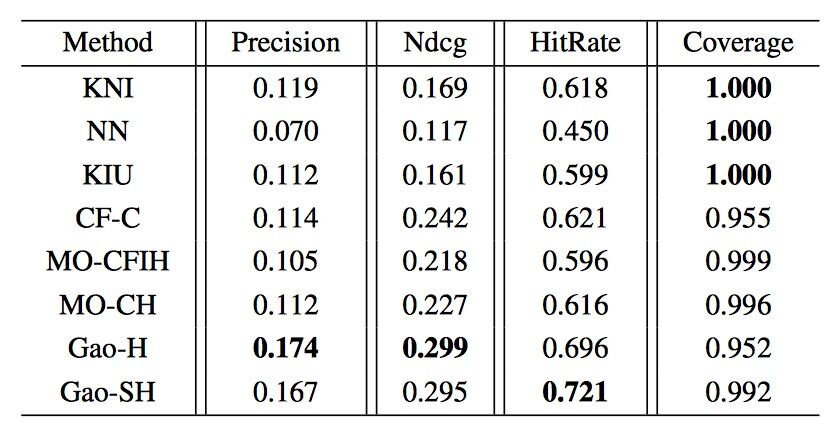
\includegraphics[width=4in]{7}
		\end{center}
		\caption{Comparison of methods}
		\label{tab:1}
	\end{figure}
	
	\section{Conclusion}
	推荐系统基于用户以前的对于物品的一些交互预测他们在未来的偏好。在已有的方法中,有很多用来推荐的技术,比如基于近邻,基于机器学习和基于矩阵分解的方法。其中一个很流行的方法便是基于矩阵分解的方法,它使用低秩矩阵对输入数据进行近似。与此相类似,在自然语言处理中的词嵌入方法也是学习输入元素在低维向量空间的表示。
	
	注意到词嵌入与矩阵分解技术的相似性,并受到之前的一些将文本处理的技术, Word2Vec的skip-gram技术应用到推荐中的方法的启发。本文工作旨在为基于以往的偏好行为为目标用户推荐top-k个地点。我使用了采集自Foursquare的数据。实验结果表明使用自然语言处理技术的确非常有效,Word2Vec的skip-gram技术对于推荐很有前景。
	
	在未来我还想进行一下改进:第一,我想利用Word2Vec的CBOW技术进行推荐,并与skip-gram技术进行比较。第二,我想扩大数据集,评测在更大数据上的一些表现。第三,由于实验表明多种特征的组合能够提高推荐表现,我想利用向量空间的表达对多种特征进行组合。
	
	%参考文献

	\bibliographystyle{plain}
	%\addcontentsline{toc}{section}{参考文献} %向目录中添加条目,以章/section的名义
	\bibliography{ref/FromWordEmbeddingsToItemRecommendation}
	
	
\end{document}